\documentclass[a4paper,11pt]{article}
\usepackage{amsfonts}
\usepackage{amssymb}
\usepackage{amsmath}
\usepackage[latin1]{inputenc}
\usepackage{graphicx}
\usepackage{soul}
\usepackage[font=small]{caption}
\usepackage{booktabs}
\usepackage{array}
\usepackage{tabularx}
\usepackage{colonequals}
\usepackage{subfigure}
\usepackage[latin,italian,english]{babel} 
\usepackage{mathtools}
\usepackage{dsfont}
\usepackage{geometry}
\geometry{a4paper,left=3cm}


\begin{document}

\begin{figure}
\centering

\includegraphics[scale=0.50]{logo.jpg}
\end{figure}

	\title{SPLINES MODULE\\ \vspace{0.5cm} IN480 course\\ \vspace{0.5cm} Curves, surfaces and splines with LAR*}
	\vspace{0.5cm}
	\author{Chiara Santorsola, Francesca Valletti}
\maketitle

\newpage
\tableofcontents
\newpage

\section{Introduction}
The \emph{Splines} library, named \texttt{splines.py} within the Python version of the LARCC framework, provides algorithms to compute curves and surfaces using spline interpolation. We are going to show the Julia translation of this package, made to simplify the development of a parallel version. In the following pages we are going to see the original package's structure, then we will study each function separately.

\subsection{Requirements}
The Julia code can run without installing further packages. It is built to manage the same types of input and output from the Python code, which implies that it should be compatible with \emph{Plasm} graphic interface.

\subsection{API}

\begin{figure}[h]
\centering
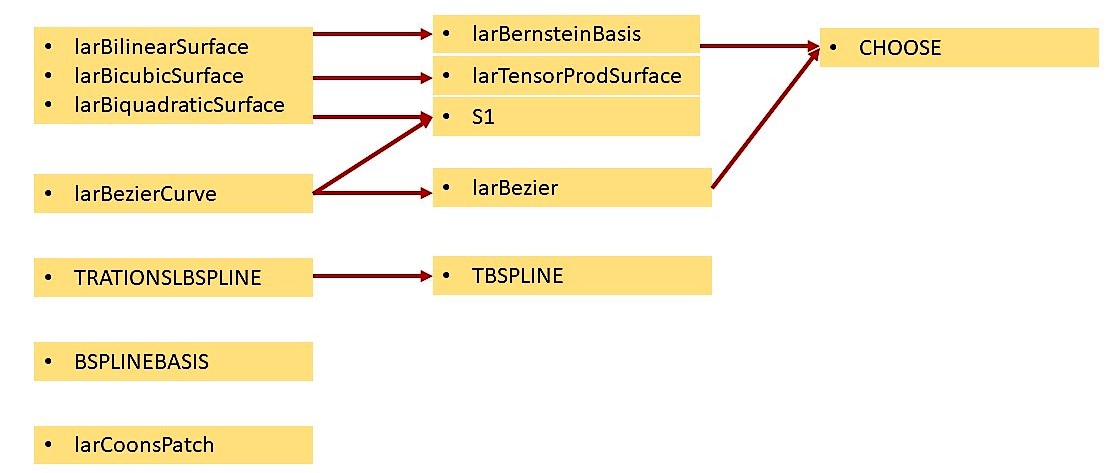
\includegraphics[scale=0.50]{grafofinale.jpg}
\caption{dependencies graph}
\end{figure}

In Julia translation the dependencies from the pyplasm function \texttt{CHOOSE} have been removed, now it is used the built-in function \texttt{binomial}.
The dependencies from the pyplasm selector \texttt{S1} are preserved introducing the \texttt{sel} function in this package (see section~\ref{sec: sel}). \\
The Julia API describes the serial functions but it is the same for the parallel ones, the only difference is the names beginning with a ``p''. \\

\emph{\texttt{larBernsteinBasis(u::Function, n::Int64)}} \\
\emph{input}: \texttt{u} is a function named selector \texttt{Sn} (see sec~\ref{sec: sel}), it takes an array and returns the n-th component; \texttt{n} is the Bernstein polynomial's degree. \\
\emph{output}:  \texttt{map\_fn} is a vector function. \\
\emph{description}: the output list is a polynimial vector function composed by the first $n+1$ elements in Bernstein basis. Those polynomials are ready to be calculated in \texttt{point}'s coordinate selected by \texttt{u} (usually the fist one, i.e. \texttt{u = sel(1)}). \\

\emph{\texttt{larBezier\{T<:Real\}(u::Function, controldata::Array\{Array\{T,1\},1\})}} \\
\emph{input}: \texttt{u} is a selector \texttt{Sn}; \texttt{controldata} is a list of $n+1$ control points. \\
\emph{output}:  \texttt{map\_fn} is a vector function, i.e. the polynomial vector function to apply to the chosen \texttt{point}. \\
\emph{description}: taken as an input $n+1$ control points, this function calculates the generic B\'ezier surface of order $n$.  \\

\emph{\texttt{larBezierCurve\{T<:Real\}(controlpoints::Array\{Array\{T,1\},1\})}} \\
\emph{input}: \texttt{cotrolpoints} is a list of arrays. \\
\emph{output}:  \texttt{map\_fn} is a vector function, i.e. the polynomial vector function to apply to the chosen \texttt{point}. \\
\emph{description}: taken as an input $n+1$ control points, this function calculates the generic B\'ezier surface of order $n$ on the first \texttt{point}'s coordinate.  \\

\emph{\texttt{larTensorProdSurface\{F<:Function, T<:Real\}(args::Array\{F, 1\},\\ controlpoints::Array\{Array\{Array\{T, 1\}, 1\}, 1\})}} \\
\emph{input}: \texttt{args} is a list of two vector functions, the bases of the two curves we want to multiply (respectively with degree $n$ and $m$); \texttt{controlpoints} is a list of $n+1$ lists of $m+1$ control points. \\
\emph{output}: \texttt{map\_fn} is a vector function, i.e. the polynomial vector function to apply to the chosen \texttt{point}. \\
\emph{description}: this function gives the tensor product of two curves, i.e. a tensor product surface. For example, if the basis are Bernstein basis we have the product between two B\'ezier curves (a B\'ezier surface).  \\

\emph{\texttt{larBilinearSurface\{T<:Real\} \\ (controlpoints::Array\{Array\{Array\{T, 1\}, 1\}, 1\})}} \\
\emph{input}: \texttt{controlpoints} is a list of two lists of control points. \\
\emph{output}: \texttt{map\_fn} is a vector function, i.e. the polynomial vector function to apply to the chosen \texttt{point}. \\
\emph{description}: this function calculates the first two Bernstein polynomials of first degree and then, with tensor product on the chosen \texttt{controlpoints}, the relative bilinear B\'ezier surface.  \\

\emph{\texttt{larBiquadraticSurface\{T<:Real\} \\ (controlpoints::Array\{Array\{Array\{T, 1\}, 1\}, 1\})}} \\
\emph{input}: \texttt{controlpoints} is a list of two lists of control points. \\
\emph{output}: \texttt{map\_fn} is a vector function, i.e. the polynomial vector function to apply to the chosen \texttt{point}. \\
\emph{description}: this function calculates the first three Bernstein polynomials of second degree and then, with tensor product on the chosen \texttt{controlpoints}, the relative biquadratic B\'ezier surface.  \\

\emph{\texttt{larBicubicSurface\{T<:Real\} \\ (controlpoints::Array\{Array\{Array\{T, 1\}, 1\}, 1\})}} \\
\emph{input}: \texttt{controlpoints} is a list of two lists of control points. \\
\emph{output}: \texttt{map\_fn} is a vector function, i.e. the polynomial vector function to apply to the chosen \texttt{point}. \\
\emph{description}: this function calculates the first four Bernstein polynomials of third degree and then, with tensor product on the chosen \texttt{controlpoints}, the relative bicubic B\'ezier surface.  \\

\emph{\texttt{larCoonsPatch\{F<:Function\}(args::Array\{F, 1\})}} \\
\emph{input}: \texttt{args} is a list of four curves. \\
\emph{output}: \texttt{map\_fn} is a vector function, i.e. the polynomial vector function to apply to the chosen \texttt{point}. \\
\emph{description}: this function takes four curves and generates the bilinearly blended Coons patch surface.  \\

\emph{\texttt{bsplineBasis\{T<:Real\}(degree::Int64, knots::Array\{T, 1\},  \\ ncontrols::Int64)}} \\
(previously called \texttt{BSPLINEBASIS}) \\
\emph{input}: \texttt{degree} is an integer (the interpolation degree); \texttt{knots} is a list of real numbers; \texttt{ncontrols} is an integer (the number of control points).\\
\emph{output}: \texttt{map\_fn} is a vector function, i.e. the polynomial vector function to apply to the chosen \texttt{point}. \\
\emph{description}: this function takes the desired interpolation degree, $p$, a list of knots and the number of control points $n+1$, checks if the number of knots is equal to $n+p+2$ and calculates a Bspline basis using De Boor coefficients, calculated recursively.  \\

\emph{\texttt{t\_bspline\{T<:Real, F<:Function\}(u::Function, \\ degree::Int64, knots::Array\{T, 1\}, points\_fn::Array\{F, 1\})}} \\
(previously called \texttt{TBSPLINE}) \\
\emph{input}: \texttt{u} is a selector \texttt{Sn}; \texttt{degree} is an integer (the interpolation degree); \texttt{knots} is a list of real numbers; \texttt{points\_fn} is a list of functions (control points are parametric curves, we apply them on the selected \texttt{point}'s coordinate).\\
\emph{output}: \texttt{map\_fn} is a vector function, i.e. the polynomial vector function to apply to the chosen \texttt{point}. \\
\emph{description}: this function takes the desired interpolation degree, $p$, a list of knots and the list of $n + 1$ control points, checks if the number of knots is equal to $n+p+2$ and calculates a transfinite B-spline segment using De Boor coefficients, calculated recursively.  \\

\emph{\texttt{t\_nurbs\{T<:Real, F<:Function\}(u::Function, \\ degree::Int64, knots::Array\{T, 1\}, points\_fn::Array\{F, 1\})}} \\
(previously called \texttt{TRATIONALBSPLINE}) \\
\emph{input}: \texttt{u} is a selector \texttt{Sn}; \texttt{degree} is an integer (the interpolation degree); \texttt{knots} is a list of real numbers; \texttt{points\_fn} is a list of functions (control points are parametric curves, we apply them on the selected \texttt{point}'s coordinate).\\
\emph{output}: \texttt{map\_fn} is a vector function, i.e. the polynomial vector function to apply to the chosen \texttt{point}. \\
\emph{description}: this function calculates a transfinite non-uniform B-spline, calling \texttt{t\_bspline} to compute it.  \\


\section{Implementation}

During the translation we put particular attention to maintain the same input and output types. 
Serial codes are very close to the originals, we only removed some nested functions, this generates different signatures.
For example if the Python code requested something like:

\begin{verbatim}
out = larFunction(sel)(degree)(controlpoints)(point) ,
\end{verbatim}

the Julia version could be more like this:

\begin{verbatim}
out = larFunction(sel, degree, contropoints)(point) .
\end{verbatim}

Even so there will be some nested functions, they are needed for recursive algorithms and/or to produce a function in output.

\subsection{Selectors \texttt{sel}}
\label{sec: sel}

Many function in this module take in input a selector function from pyplasm package. This selectors simply take in input an integer \texttt{n} giving in output a function which in turn takes a list and returns the n-th component. So \texttt{S1} gives the first component of the input list and so on. Our translation in Julia is useful for testing function with input \texttt{u} that is one of those \texttt{Sn}.

\subsubsection{Python code}

\begin{verbatim}
def SEL(n):
    return lambda lista: lista[int(n)-1]

S1 = SEL(1)
S2 = SEL(2)
S3 = SEL(3)
\end{verbatim}

\subsubsection{Julia code}

\begin{verbatim}
function sel(n::Int64)
     return list -> list[n]
end

S1 = sel(1)
S2 = sel(2)
S3 = sel(3)
\end{verbatim}

\subsubsection{Examples}

\begin{verbatim}
v = [1.0,3.4,5.5,6.9,2.4,8.0]
fv = [[1,2,4],[2,3,5],[3,5,6],[4,5,7],[5,7,8],[6,8,9]]
@testset "sel" begin
    @test sel(4)(v) == 6.9
    @test sel(5)(fv) == [5,7,8]
\end{verbatim}


\subsection{\texttt{larBernsteinBasis}}

This function computes the vector function composed by the first $n+1$ elements in \emph{Bernstein basis}, i.e. the polynomials

\begin{equation}
\label{eqn: bernstein}
B_i^n(t)\coloneqq\binom{n}{i}(1-t)^{n-i}t^i \;\;\;\; for \; i=0,...,n\;.
\end{equation}

Those polynomials are ready to be calculated in \texttt{point}'s coordinate selected by the \texttt{u} input. They are meant to be combined with the vertices of the so called \emph{control polygon} in order to produce a \emph{B\'ezier curve} of n-th degree, as we will see later in \texttt{larBezier}'s section. \\


\subsubsection{Python code}
\begin{verbatim}
def larBernsteinBasis(U):
    def BERNSTEIN0(N):
        def BERNSTEIN1(I):
            def map_fn(point):
                t = U(point)
                out = CHOOSE([N,I])*math.pow(1-t,N-I)*math.pow(t,I)
                return out
            return map_fn
        return [BERNSTEIN1(I) for I in range(0,N+1)]
    return BERNSTEIN0
\end{verbatim}

\subsubsection{Julia serial code}

\begin{verbatim}
function larBernsteinBasis(u::Function, n::Int64)
    function map_fn(x::Array{Float64,1})
        bernstein(i, n, t::Float64) = binomial(n,i)*(1-t)^(n-i)*t^i
        return [bernstein(i, n, u(x)) for i in 0:n]
    end
    return map_fn
end
\end{verbatim}

\subsubsection{Julia parallel code}
---

\subsubsection{Unit tests code}

\paragraph{serial test}
\begin{verbatim}
@testset "larBernsteinBasis" begin
    bernstein = larBernsteinBasis(S1, 3)
    point = [0.7, 2, 7.3]
    result = bernstein(point)
    @test typeof(result) == Array{Float64,1}
end
\end{verbatim}

\paragraph{parallel test}
\begin{verbatim}
-
\end{verbatim}

\subsection{\texttt{larBezier}}
A \emph{polynomial curve} is a function that better fits a set of points given as input.
We are now assembling Bernstein polynomials to build the most important polynomial curve: the \emph{B\'ezier Curve}. \\
Given $n+1$ vertices $P_i$, called \emph{control points}, it is defined on the interval $I=[0,1]$ the B\'ezier Curve of n-th degree as the linear combination between the control points $P_i$ and their weights $B_i^n(t)$ defined in~\eqref{eqn: bernstein}.

\begin{equation*}
c(t)=\sum_{i=0}^nP_i B_i^n(t) \;\;\;\;\;\;\;\; t\in [0,1]
\end{equation*}

Bernstein's polynomials have an important feature: their sum is always equal to $1$. This means that is it sufficient to transform the vertices of control polygon in order to transform by affinity the whole curve.
In order to work with B\'ezier curves is useful to keep in mind some properties:
\begin{itemize}
\item the interval of the curve is always $I=[0,1]$;
\item the curve's starting point is $P_0$ and the ending point is $P_n$, all the other control points are not elements of the curve;
\item the convex polygon that contains the control points also contains the whole B\'ezier curve;
\item mapping the control points with an affine transformation produces the same transformation in the curve;
\item it is not possible generate circular curves;
\item to merge two different curves they have to be of the same degree.
\end{itemize}

\subsubsection{Python code}

\begin{verbatim}
def larBezier(U):
    def BEZIER0(controldata_fn):
        N = len(controldata_fn) - 1
        def map_fn(point):
            t = U(point)
            controldata = [fun(point) if callable(fun) else fun
                          for fun in controldata_fn]
            out = [0.0 for i in range(len(controldata[0]))]
            for I in range(N+1):
                weight = CHOOSE([N,I])*math.pow(1-t,N-I)*math.pow(t,I)
                for K in range(len(out)): 
                    out[K] += weight*(controldata[I][K])
            return out
        return map_fn
    return BEZIER0
\end{verbatim}

\subsubsection{Julia code}

\begin{verbatim}
function larBezier{T<:Real}(u::Function, 
          controldata::Array{Array{T,1},1})
    n = length(controldata) - 1
    dim = length(controldata[1])
    function map_fn(point::Array{Float64, 1})
        t = u(point)
        out = zeros(Float64, dim)
        for i in 0:n
            weight = bernstein(i, n)(t)
            for k in 1:dim
                out[k] += weight*controldata[i+1][k]
            end
        end
        return out
    end
    return map_fn
end
\end{verbatim}


\subsubsection{Julia parallel code}
---

\subsubsection{Unit tests code}

\paragraph{serial test}
\begin{verbatim}
@testset "larBezier" begin
    controldata = [[-0,0],[1,0],[1,1],[2,1],[3,1]]
    point = [0.5, 0.7]
    u = S2
    bezier = larBezier(u, controldata)
    result = bezier(point)
    @test typeof(result) == Array{Float64,1}
    @test length(result) == 2
end
\end{verbatim}

\paragraph{parallel test}
\begin{verbatim}
-
\end{verbatim}


\subsection{\texttt{larBezierCurve}}
This function just applies \texttt{larBezier} setting $\texttt{u} = \texttt{S1}$.

\subsubsection{Python code}

\begin{verbatim}
def larBezierCurve(controlpoints):
    return larBezier(S1)(controlpoints)
\end{verbatim}

\subsubsection{Julia code}

\begin{verbatim}
function larBezierCurve{T<:Real}(controlpoints::Array{Array{T,1},1})
    return larBezier(S1, controlpoints)
end
\end{verbatim}

\subsubsection{Julia parallel code}

-

\subsubsection{Unit tests code}

\paragraph{serial test}
\begin{verbatim}
@testset "larBezierCurve" begin
    controls = [[0,1],[0,0],[1,1],[1,0]]
    point = [0.2, 0.7]
    bezier = larBezierCurve(controls)
    result = bezier(point)
    @test typeof(result) == Array{Float64,1}
    @test length(result) == 2
end
\end{verbatim}

\paragraph{parallel test}
\begin{verbatim}
-
\end{verbatim}


\subsection{\texttt{larTensorProdSurface}}

We saw how to compute polynomial curves as linear combination between a set of control points and a basis for polynomial function in one variable. Analogously, polynomial surfaces are linear combination of control points with a suitable basis of polynomial function in \emph{two} variables. Such bivariate basis is obtained through the \emph{tensor product} between two univariate bases. That's why this kind of surfaces are called \emph{Tensor Product Surfaces}. For example a \emph{B\'ezier Surface} of degree $(n,m)$ is defined as the linear combination of two Bernstein basis, $\{B_i^n(t)\}_{i=0,...,n}$ and $\{B_j^m(t)\}_{j=0,...,n}$, with a set of $(n+1)(m+1)$ controlpoints, $P_{i,j}$:

\begin{equation*}
\label{eqn: tensorprod}
S(u,v) =\sum_{i=0}^n\sum_{j=0}^m B_i^n(u) B_j^m(v) P_{i,j}\;\;\;\;\;\;\;\; (u,v)\in [0,1]^2 \;.
\end{equation*}

The properties of tensor product surfaces are a straightforward extension of properties of the relative parametric curves.
Note that the Python code is made to take \texttt{controlpoints\_fn} that could be an array of arrays of points or vector functions. This feature was not requested in our project so the Julia translation takes \texttt{controlpoint} that is simply an array of array of points (arrays). See section~\ref{sec: fi} to see a possible solution to overcome this limitation. \\
An other difference is that we commented one of the \texttt{for} cycles in \texttt{m}, we found that it was incorrect to iterate two times on \texttt{ret}'s index. \\
Be careful: cardinality of control points must be compatible with the bases' degrees, or \texttt{larTensorProdSurface} won't work. As you can see we inserted an \texttt{error} in Julia code to warn incautious users.


\subsubsection{Python code}

\begin{verbatim}
def larTensorProdSurface(args):
    ubasis, vbasis = args
    def TENSORPRODSURFACE0(controlpoints_fn):
        def map_fn(point):
            u, v = point
            U = [f([u]) for f in ubasis]
            V = [f([v]) for f in vbasis]
            controlpoints = [f(point) if callable(f) else f 
                for f in controlpoints_fn]
            target_dim = len(controlpoints[0][0])
            ret = [0 for x in range(target_dim)]
            for i in range(len(ubasis)):
                for j in range(len(vbasis)):
                    for M in range(len(ret)):
                        for M in range(target_dim):
                            ret[M] += U[i]*V[j] * controlpoints[i][j][M]
            return ret
        return map_fn
    return TENSORPRODSURFACE0
\end{verbatim}

\subsubsection{Julia code}
   
\begin{verbatim}
function larTensorProdSurface{F<:Function, T<:Real}(args::Array{F, 1}, 
                            controlpoints::Array{Array{Array{T, 1}, 1}, 1})
    ubasis , vbasis = args
    function map_fn(point::Array{Float64, 1})
        u, v = point
        ub = ubasis([u])
        vb = vbasis([v])
        target_dim = length(controlpoints[1][1])
        ret = zeros(Float64, target_dim)
        dim_u = length(ub)
        dim_v = length(vb)
        if (length(controlpoints)!= dim_u || length(controlpoints[1])!= dim_v)
            error("Invalid set of control points for those bases!") 
        end
        for i in 1:dim_u
            for j in 1:dim_v
                for m in 1:target_dim
                    #for m in 1:target_dim 
                        ret[m] += ub[i]*vb[j]*controlpoints[i][j][m]
                    #end
                end
            end
        end
        return ret
    end
    return map_fn
end
\end{verbatim}

\subsubsection{Julia parallel code}
---

\subsubsection{Unit tests code}

\paragraph{serial test}
\begin{verbatim}
@testset "larTensorProdSurface" begin
    controlpoints = [[[0,0,0],[2,-4,2],[3,1,-1]],
                 [[0,3,1],[4,0,0],[4,2,-4]],
                 [[2,0,3],[0,5,1],[1,0,-4]],
                 [[3,0,2],[-1,-1,-1],[2,3,0]],
                 [[2,-1,0],[0,-4,1],[3,3,-3]]]
    basis1 = larBernsteinBasis(S1, 4) 
    basis2 = larBernsteinBasis(S1, 2) 
    point = [0.5, 0.2]
    tensorprodsurf = larTensorProdSurface([basis1, basis2], controlpoints)
    result = tensorprodsurf(point)
    @test typeof(result) == Array{Float64,1}
    @test length(result) == 3
end
\end{verbatim}

\paragraph{parallel test}
\begin{verbatim}
-
\end{verbatim}


\subsection{\texttt{larBilinearSurface}}

Taken in input two control points, this function calculates two Bernstein bases of first degree and then, with tensor product, the relative Bilinear B\'ezier surface.

\subsubsection{Python code}

\begin{verbatim}
def larBilinearSurface(controlpoints):
    basis = larBernsteinBasis(S1)(1)
    return larTensorProdSurface([basis, basis])(controlpoints)
\end{verbatim}

\subsubsection{Julia code}

\begin{verbatim}
function larBilinearSurface{T<:Real}(controlpoints::Array{Array{Array{T, 1}, 1}, 1})
    basis = larBernsteinBasis(S1, 1)
    return larTensorProdSurface([basis, basis], controlpoints)
end
\end{verbatim}

\subsubsection{Julia parallel code}
---

\subsubsection{Unit tests code}

\paragraph{serial test}
\begin{verbatim}
@testset "larBilinearSurface" begin
    controlpoints = [[[0,0,0],[2,-4,2]],[[0,3,1],[4,0,0]]]
    point = [0.5,0.7]
    bilinear = larBilinearSurface(controlpoints)
    result = bilinear(point)
    @test typeof(result) == Array{Float64,1}
    @test length(result) == 3
end
\end{verbatim}

\paragraph{parallel test}
\begin{verbatim}
-
\end{verbatim}


\subsection{\texttt{larBiquadraticSurface}}

Taken in input three control points, this function calculates two Bernstein bases of second degree and then, with tensor product, the relative Biquadratic B\'ezier surface.

\subsubsection{Python code}

\begin{verbatim}
def larBiquadraticSurface(controlpoints):
    basis1 = larBernsteinBasis(S1)(2)
    basis2 = larBernsteinBasis(S1)(2)
    return larTensorProdSurface([basis1, basis2])(controlpoints)
\end{verbatim}

\subsubsection{Julia code}

\begin{verbatim}
function larBiquadraticSurface{T<:Real}(controlpoints::Array{Array{Array{T, 1}, 1}, 1})
    basis1 = larBernsteinBasis(S1, 2)
    basis2 = larBernsteinBasis(S1, 2)
    return larTensorProdSurface([basis1, basis2], controlpoints)
end
\end{verbatim}

\subsubsection{Julia parallel code}
---

\subsubsection{Unit tests code}

\paragraph{serial test}
\begin{verbatim}
@testset "larBiquadraticSurface" begin
    controlpoints = [[[0,0,0],[2,0,1],[3,1,1]],
               [[1,3,-1],[2,2,0],[3,2,0]],
               [[-2,4,0],[2,5,1],[1,3,2]]]
    biquadratic = larBiquadraticSurface(controlpoints)
    point = [0.7, 0.2]
    result = biquadratic(point)
    @test typeof(result) == Array{Float64,1}
    @test length(result) == 3
end
\end{verbatim}

\paragraph{parallel test}
\begin{verbatim}
-
\end{verbatim}

\subsection{\texttt{larBicubicSurface}}

Taken in input four control points, this function calculates two Bernstein bases of third degree and then, with tensor product, the relative Bicubic B\'ezier surface.

\subsubsection{Python code}

\begin{verbatim}
def larBicubicSurface(controlpoints):
    basis1 = larBernsteinBasis(S1)(3)
    basis2 = larBernsteinBasis(S1)(3)
    return larTensorProdSurface([basis1, basis2])(controlpoints)
\end{verbatim}

\subsubsection{Julia code}

\begin{verbatim}
function larBicubicSurface{T<:Real}(controlpoints::Array{Array{Array{T, 1}, 1}, 1})
    basis1 = larBernsteinBasis(S1, 3)
    basis2 = larBernsteinBasis(S1, 3)
    return larTensorProdSurface([basis1, basis2], controlpoints)
end
\end{verbatim}

\subsubsection{Julia parallel code}
---

\subsubsection{Unit tests code}

\paragraph{serial test}
\begin{verbatim}
@testset "larBicubicSurface" begin
    controlpoints = [[[0,0,0], [0,3,4], [0,6,3], [0,10,0]],
                     [[3,0,2], [2,2.5,5], [3,6,5], [4,8,2]],
                     [[6,0,2], [8,3,5], [7,6,4.5], [6,10,2.5]],
                     [[10,0,0], [11,3,4], [11,6,3], [10,9,0]]]
    bicubic = larBicubicSurface(controlpoints)
    point = [0.7,0.2]
    result = bicubic(point)
    @test typeof(result) == Array{Float64,1}
    @test length(result) == 3
end
\end{verbatim}

\paragraph{parallel test}
\begin{verbatim}
-
\end{verbatim}


\subsection{\texttt{larCoonsPatch}}

A \emph{Coons Patch} si a type of manifold parameterization used to smoothly join other surfaces together. Given four curves $c_0(u)$, $c_1(u)$, $d_0(v)$ and $d_1(v)$ which meet at four corners (i.e. $c_0(0)=d_0(0)$, $c_0(1)=d_1(0)$, $c_1(0)=d_0(1)$ and $c_1(1)=d_1(1)$), linear interpolation between $c_0$ and $c_1$ and between $d_0$ and $d_1$ produces two ruled surfaces defined in $[0,1]^2$:

\begin{align*}
L_c(u,v)=(1-v)c_0(u)+vc_1(u) \;,  \\
L_d(u,v)=(1-u)d_0(v)+ud_1(v)\;.
\end{align*}

The bilinear interpolation on the four corner points is another surface:

\begin{equation*}
B(u,v)=c_0(0)(1-u)(1-v)+c_0(1)u(1-v)+c_1(0)(1-u)v+c_1(1)uv \;.
\end{equation*}

The resulting bilinearly blended Coons patch is the surface:

\begin{equation*}
C(u,v)=L_c(u,v)+L_d(u,v)-B(u,v) \; .
\end{equation*}

This function takes four curves, for example four B\'ezier curves, and generates their Coons patch surface. \\
Differences between Python and Julia code are evident, Python checks if the arguments are functions inside the nested \texttt{map\_fn} function, Julia instead have input typed, so the function expects a list of functions in input.

\subsubsection{Python code}

\begin{verbatim}
def larCoonsPatch(args): 
    su0_fn , su1_fn , s0v_fn , s1v_fn = args
    def map_fn(point):
        u, v = point
        su0 = su0_fn(point) if callable(su0_fn) else su0_fn
        su1 = su1_fn(point) if callable(su1_fn) else su1_fn
        s0v = s0v_fn(point) if callable(s0v_fn) else s0v_fn
        s1v = s1v_fn(point) if callable(s1v_fn) else s1v_fn
        ret = [0.0 for i in range(len(su0))]
        for K in range(len(ret)):
            ret[K] = ((1-u)*s0v[K] + u*s1v[K] + (1-v)*su0[K] + v*su1[K] 
                + (1-u)*(1-v)*s0v[K] + (1-u)*v*s0v[K] + u*(1-v)*s1v[K] 
                + u*v*s1v[K])
        return ret
    return map_fn
\end{verbatim}

\subsubsection{Julia code}

\begin{verbatim}
function larCoonsPatch{T<:Function}(args::Array{T, 1})
    su0_fn , su1_fn , s0v_fn , s1v_fn = args
    function map_fn(point)
        u, v = point
        su0 = su0_fn(point)
        su1 = su1_fn(point)
        s0v = s0v_fn(point)
        s1v = s1v_fn(point)
        ret = zeros(Float64, length(su0))  
        for k in 1:length(ret)
            ret[k] = ((1-u)*s0v[k] + u*s1v[k]+(1-v)*su0[k] + v*su1[k] 
                + (1-u)*(1-v)*s0v[k] + (1-u)*v*s0v[k] + u*(1-v)*s1v[k] 
                + u*v*s1v[k])
        end
        return ret
    end
    return map_fn
end
\end{verbatim}

\subsubsection{Julia parallel code}
---

\subsubsection{Unit tests code}

\paragraph{serial test}
\begin{verbatim}
@testset "larCoonsPatch" begin
    Su0 = larBezier(S1, [[0,0,0],[10,0,0]])
    Su1 = larBezier(S1, [[0,10,0],[2.5,10,3],[5,10,-3],[7.5,10,3],[10,10,0]])
    Sv0 = larBezier(S2, [[0,0,0],[0,0,3],[0,10,3],[0,10,0]])
    Sv1 = larBezier(S2, [[10,0,0],[10,5,3],[10,10,0]])
    point = [0.7, 0.2]
    coons = larCoonsPatch([Su0,Su1,Sv0,Sv1])
    result = coons(point)
    @test typeof(result)==Array{Float64,1}
end
\end{verbatim}

\paragraph{parallel test}
\begin{verbatim}
-
\end{verbatim}


\subsection{\texttt{bsplineBasis}}

\emph{Spline Curves} are curves composed by other curves. They are built joining polynomial curves preserving continuity and, eventually, smoothness. We are going to show a function that computes \emph{B-splines} which are particular spline functions that require minimal support with respect to a given degree, smoothness and domain partition. \\
Let's consider an interval $I=[a,b]$ and a non-decreasing sequence of $n+1$ real numbers in it $a=t_0 \leq t_1 \leq ... \leq t_n=b$, called \emph{knots sequence}. In each subinterval it is defined a polynomial, to do so we can use the \emph{Cox-de Boor recursion formula}. B-splines of order 1 are defined by

\begin{equation*}
B_{i,1}(t)\coloneqq
\left\{
	\begin{array}{ll}
	1 \;\;\;\; if \; t_i \leq t \leq t_{i+1} \;, \\
	0 \;\;\;\; otherwise \;,
	\end{array}
	\right.
\end{equation*}

and higher order B-splines are defined by

\begin{equation*}
B_{i,k+1}(t)\coloneqq\frac{t-t_i}{t_{i+k}-t_i}B_{i,k}(t)+\frac{t_{i+k+1}-t}{t_{i+k+1}-t_{i+1}}B_{i+1,k}(t) \;.
\end{equation*}

When the knots are distinct, the first $n-1$ derivatives of the polynomial pieces are continuous across each knot. When $r$ knots are coincident, only the first $n-r$ derivative of the spline are continuous across that knot. If the length of the subintervals defined by such knots is constant the spline is called \emph{uniform}, but it may vary, in this case we have \emph{non-uniform} splines. \\
Once we built a B-spline basis, we can compute a parametric curve defined by a given set of $m+1$ control points $P_i=(x_i,y_i)$ in 2D space or $P_i=(x_i,y_i,z_i)$ in 3D space. The curve will be of the form

\begin{equation*}
C(t)=(\sum_{i=0}^n x_iB_{i,k}(t), \sum_{i=0}^n y_iB_{i,k}(t), \sum_{i=0}^n z_iB_{i,k}(t)) \;.
\end{equation*}

If $k$ is the degree of the B-basis functions, the spline degree is $h=k+1$. The relation $m=n+k$ must hold. \\
Those kind of curve have the same property of Bezier curves: if the control points are all transformed by affine transformation, then the corresponding curve is transformed in the same way.

\subsubsection{Python code}

\begin{verbatim}
def BSPLINEBASIS(degree):
    def BSPLINE0(knots):
        def BSPLINE1(ncontrols):
            n = ncontrols - 1
            m = len(knots) - 1
            k = degree + 1
            T = knots
            tmin, tmax = T[k-1], T[n+1]
            if len(knots) != (n+k+1):
	         raise Exception("Invalid point/knots/degree for bspline!")
            def N(i,k,t):
                if k == 1:
                    if(t>=T[i] and t<T[i+1]) 
                        or (t==tmax and t>=T[i] and t<=T[i+1]):
                        return 1
                    else:
                        return 0
                ret = 0
                num1, div1 = t - T[i], T[i+k-1] - T[i]
                if div1 != 0: ret += (num1/div1) * N(i,k-1,t)
                num2, div2 = T[i+k] - t, T[i+k] - T[i+1]
                if div2 != 0: ret += (num2/div2) * N(i+1,k-1,t)
                return ret
            def map_fn(point):
                t = point[0]
                return [N(i,k,t) for i in range(n+1)]
            return map_fn
        return BSPLINE1
    return BSPLINE0
\end{verbatim}

\subsubsection{Julia code}

\begin{verbatim}
function bsplineBasis{T<:Real}(degree::Int64, knots::Array{T,1}, ncontrols::Int64)
    n = ncontrols - 1
    m = length(knots) - 1
    k = degree + 1
    tmin, tmax = knots[k-1], knots[n+1]       
    if length(knots)!=(n+k+1) 
        error("Invalid point/knots/degree for bspline!") 
    end
    # de Boor coefficients
    function deBoor(i::Int64, k::Int64, t::Float64)           
        # deBoor coefficient Ni1(t)
        if k == 1
            if(t >= knots[i] && t<knots[i+1]) 
                || (t == tmax && t>=knots[i] && t<=knots[i+1])
                return 1
            else
                return 0
            end
        end
        # deBoor coefficient Nik(t)
        ret = 0    
        num1, div1 = t-knots[i], knots[i+k-1]-knots[i]
        if div1 != 0 
            ret += (num1/div1) * deBoor(i,k-1,t) 
        end
        num2, div2 = knots[i+k]-t, knots[i+k]-knots[i+1]
        if div2 != 0
            ret += (num2/div2) * deBoor(i+1,k-1,t)
        end
        return ret
    end
    # map function
    function map_fn{T<:Real}(point::Array{T, 1})
        t = point[1]
        return [deBoor(i, k, t) for i in 1:(n+1)]
    end
    return map_fn
end
\end{verbatim}

\subsubsection{Julia parallel code}
---

\subsubsection{Unit tests code}

\paragraph{serial test}
\begin{verbatim}
@testset "bsplineBasis" begin
    knots = [0,0,0,0,1,2,3,4,4,4,4]
    ncontrols = 8
    degree = 2
    basis = bsplineBasis(degree, knots, ncontrols)
    point = [0.7,0.2,3.0]
    result = basis(point)
    @test typeof(result) == Array{Float64,1}
    @test length(result) == 9
end
\end{verbatim}

\paragraph{parallel test}
\begin{verbatim}
-
\end{verbatim}

\subsection{\texttt{t\_bspline}}

The ``\texttt{t}'' in this function's name stands for \emph{transfinite}, which means that the interpolation works with a non-numerable set of control points, in particular controls we use are curves. In fact, it's easy to see that it expects the \texttt{point\_fn} input to be an array of functions.

\subsubsection{Python code}
\begin{verbatim}
def TBSPLINE(U):
    def TBSPLINE0(degree):
        def TBSPLINE1(knots):
            def TBSPLINE2(points_fn):

                n = len(points_fn) - 1
                m = len(knots) - 1
                k = degree + 1
                T = knots
                tmin, tmax = T[k-1], T[n+1]

                if len(knots) != (n+k+1):
                   raise Exception("Invalid point/knots/degree for bspline!")
   
                    # de boord coefficients
                    def N(i, k, t):
   
                        # Ni1(t)
                        if k == 1: 
                            if(t>=T[i] and t<T[i+1]) 
                                or (t==tmax and t>=T[i] and t<=T[i+1]): 
                            # i use strict inclusion for the max value
                                return 1
                            else:
                                return 0
   
                        # Nik(t)
                        ret = 0
   
                        num1, div1 = t-T[i], T[i+k-1]-T[i]  
                        if div1 != 0: ret += (num1/div1) * N(i, k-1, t)
                        # elif num1 != 0: ret += N(i, k-1, t)
   
                        num2, div2 = T[i+k]-t, T[i+k]-T[i+1]
                        if div2 != 0:  ret += (num2/div2) * N(i+1, k-1, t)
                        # elif num2 != 0: ret += N(i, k-1, t)
   
                        return ret
   
                        # map function
                    def map_fn(point):
                        t = U(point)
   
                        # if control points are functions
                        points = [f(point) if callable(f) else f for f in points_fn]
   
                        target_dim = len(points[0])
                        ret = [0 for i in range(target_dim)];
                        for i in range(n+1):
                            coeff=N(i, k, t) 
                            for M in range(target_dim):
                                ret[M] += points[i][M] * coeff
                        return ret
   
                    return map_fn
                return TBSPLINE2
            return TBSPLINE1
        return TBSPLINE0
\end{verbatim}

\subsubsection{Julia code}

\begin{verbatim}
function t_bspline{T<:Real, F<:Function}(u::Function, 
                  degree::Int64, knots::Array{T,1}, points_fn::Array{F, 1})
   
    n = length(points_fn)-1
    m = length(knots)-1
    k = degree + 1
    tmin, tmax = knots[k-1], knots[n+1]
    if length(knots)!=(n+k+1) 
        error("Invalid point/knots/degree for bspline!") 
    end
    # de Boor coefficients
    function deBoor(i::Int64, k::Int64, t::Float64)
        # Ni1(t)
        if k == 1 
            if(t>=knots[i] && t<knots[i+1]) 
                || (t==tmax && t>=knots[i] && t<=knots[i+1])
                # i use strict inclusion for the max value
                return 1
            else
                return 0
            end
        end
        # Nik(t)
        ret = 0
        
        num1, div1 = t-knots[i], knots[i+k-1]-knots[i]  
        if div1 != 0 
            ret += (num1/div1) * deBoor(i, k-1, t)
            # elif num1 != 0: ret += deBoor(i, k-1, t)
        end
        
        num2, div2 = knots[i+k]-t, knots[i+k]-knots[i+1]
        if div2 != 0  
            ret += (num2/div2) * deBoor(i+1, k-1, t)
            # elif num2 != 0: ret += deBoor(i, k-1, t)
        end
           
        return ret
    end
    
    # map function
    function map_fn(point::Array{Float64, 1})
        t = u(point)
        target_dim = length(points_fn[1](point))
        ret = zeros(Float64, target_dim)
        for i in 1:n+1
            coeff = deBoor(i,k,t) 
            for m in 1:target_dim
                ret[m] += points_fn[i](point)[m] * coeff
            end
        end
        return ret
    end
    return map_fn
end
\end{verbatim}

\subsubsection{Julia parallel code}
---

\subsubsection{Unit tests code}

\paragraph{serial test}
\begin{verbatim}
@testset "t_bspline" begin
    b1 = larBezier(S1, [[0,1,0],[0,1,5]])
    b2 = larBezier(S1, [[0,0,0],[0,0,5]])
    b3 = larBezier(S1, [[1,0,0],[2,-1,2.5],[1,0,5]])
    b4 = larBezier(S1, [[1,1,0],[1,1,5]])
    b5 = larBezier(S1, [[0,1,0],[0,1,5]])
    controls = [b1, b2, b3, b4, b5]
    #knots = [0,1,2,3,4,5,6,7]           # periodic B-spline
    knots = [0,0,0,1,2,3,3,3]           # non-periodic B-spline
    tbspline = t_bspline(S2, 2, knots, controls) 
    result = tbspline([0.7, 0.2])
    @test typeof(result) == Array{Float64,1}
    @test length(result) == 3
end
\end{verbatim}

\paragraph{parallel test}
\begin{verbatim}
-
\end{verbatim}


\subsection{\texttt{t\_nurbs}}

The last function's name stands for \emph{transfinite Non-Uniform Rational Basis-Spline}. We already saw what \emph{transfinite} and \emph{non-uniform} mean, let's take a look at the construction of this kind of splines to understand why they are called \emph{rational}. \\
A rational B-spline segment $R_i(t)$ is defined as the projection from the origin on the hyperplane $x_{d+1}=1$ of a polynomial B-spline segment $C_i(u)$ in $\mathds{E}^{d+1}$ homogeneous space, it means it can be written as

\begin{equation*}
R_i(t)=\sum_{l=0}^k w_{i-l} P_{i-l} \frac{B_{i-l,k+1}(t)}{w(t)}
\end{equation*}

with $k \leq i \leq m$, $t \in [t_i, t_{i+1})$ and $w(t)=\sum_{l=0}^k w_{i-l}B_{i-l,k+1}(t)$. \\
In the following code they are computed as non-uniform B-splines by using homogeneous control points and simply by dividing the Cartesian coordinates times the homogeneous one, how it's easy to see.

\subsubsection{Python code}
\begin{verbatim}
def TRATIONALBSPLINE(U):
    def TRATIONALBSPLINE0(degree):
       def TRATIONALBSPLINE1(knots):
           def TRATIONALBSPLINE2(points):
               bspline = TBSPLINE(U)(degree)(knots)(points)
               def map_fn(point):
                   ret = bspline(point)
                   last = ret[-1]
                   if last != 0: ret = [value/last for value in ret]
                   ret = ret[:-1]
                   return ret
               return map_fn
           return TRATIONALBSPLINE2
       return TRATIONALBSPLINE1
    return TRATIONALBSPLINE0
\end{verbatim}

\subsubsection{Julia code}

\begin{verbatim}
function t_nurbs{T<:Real, F<:Function}(u::Function, 
                  degree::Int64, knots::Array{T,1}, points::Array{F, 1})
    bspline = t_bspline(u, degree, knots, points)
    function map_fn(point)
        ret = bspline(point)
        last = ret[end]    #last element in ret
        if last != 0
            ret = [value/last for value in ret]
        end
        ret = ret[1:end-1]    #it slices off the last element (that is now = 1)
        return ret
    end
    return map_fn
end
\end{verbatim}

\subsubsection{Julia parallel code}
---

\subsubsection{Unit tests code}

\paragraph{serial test}
\begin{verbatim}
@testset "t_nurbs" begin
    knots = [0,0,0,1,1,2,2,3,3,4,4,4]
    p = sqrt(2)/2.0
    controls = [[-1,0,1], [-p,p,p], [0,1,1], [p,p,p],[1,0,1], [p,-p,p],[0,-1,1], [-p,-p,p], [-1,0,1]]
    c1 = larBezier(S1, [[-1,0,0,1],[-1,0,1,1]])
    c2 = larBezier(S1, [[-p,p,0,p],[-p,p,p,p]])
    c3 = larBezier(S1, [[0,1,0,1],[0,1,1,1]])
    c4 = larBezier(S1, [[p,p,0,p],[p,p,p,p]])
    c5 = larBezier(S1, [[1,0,0,1],[1,0,1,1]])
    c6 = larBezier(S1, [[p,-p,0,p],[p,-p,p,p]])
    c7 = larBezier(S1, [[0,-1,0,1],[0,-1,1,1]])
    c8 = larBezier(S1, [[-p,-p,0,p],[-p,-p,p,p]])
    c9 = larBezier(S1, [[-1,0,0,1],[-1,0,1,1]])
    controls = [c1,c2,c3,c4,c5,c6,c7,c8,c9]         
    tnurbs = t_nurbs(S2,2,knots,controls)
    result = tnurbs([0.7, 0.2])
    @test typeof(result) == Array{Float64,1}
    @test length(result) == 3
end
\end{verbatim}

\paragraph{parallel test}
\begin{verbatim}
-
\end{verbatim}

\section{Conclusions}

\subsection{Further Implementation}
\label{sec: fi}
Some function in Python code had the possibility to accept functions or points in input (as control points). That was not requested in our project, but it can be done also in Julia. An idea to replicate this in a stable way is to construct a function that takes constant arrays and converts them in constant vector functions, then use those function as inputs, just as transfinite functions actually do. In this way Julia doesn't have to deal with different Types of input.

\end{document}
